\section{Example \& applications}

\begin{figure*}
\label{fig:ihierarchy}
\centering
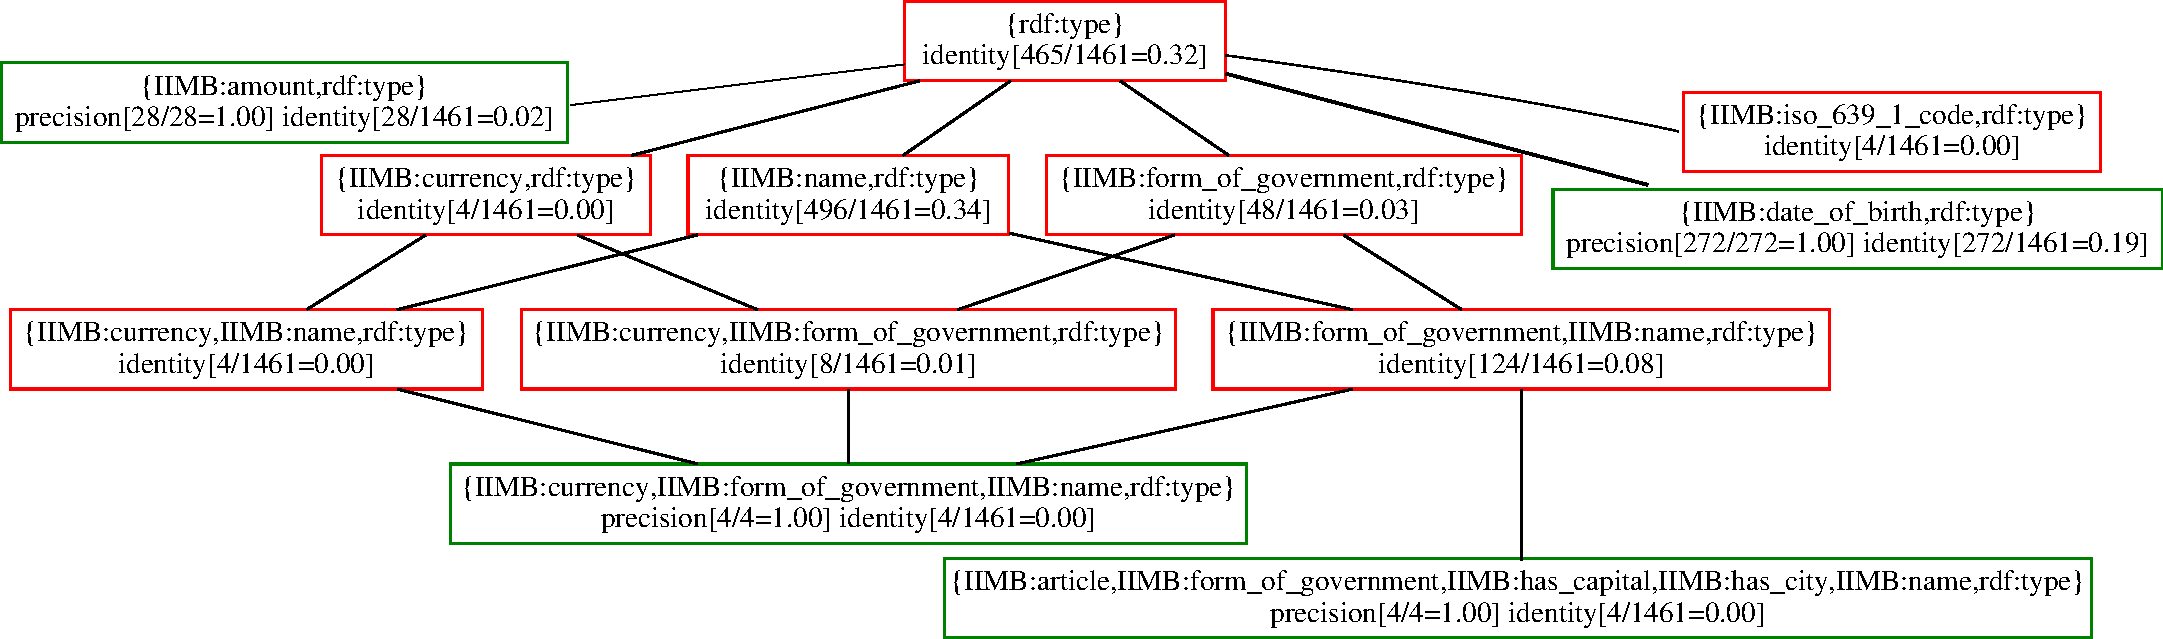
\includegraphics[width=\textwidth]{./img/iimb_16}
\caption{...}
\end{figure*}

Figure 1 shows an example of the lower and higher
  approximations for a data- and linkset of the IIMB database.
Each rectangular box represents an identity sub-relation.
Since in this figure a partition is only drawn when there is at least one
  identity pair that is indiscernible with respect to some set of
  predicates, the higher approximation amounts to the entire figure.
The lower approximation only consists of those partition sets that contain
  at least one identity pair, and that contain no non-identity pair;
  these are distinguished by green borders.
ADD PRECISION CALCULATIONS FOR ALL IDENTITY SUB-RELATIONS

\subsection{Applications}

The precision of an identity subrelation is defined as
    the number of identity pairs in the subrelation
  divided by
    the number of pairs in the subrelation.

This approximation of the identity relation allows us to
  give suggestions about which pairs to in/exclude from
  an identity relation, and
  gives an indicator for the quality of an identity relation.

